\documentclass[a4paper]{exam}

\usepackage[ruled,linesnumbered]{algorithm2e}
\usepackage{algpseudocode}
\usepackage{geometry}
\usepackage{tikz}
\usepackage{xcolor}
\usetikzlibrary{shapes.geometric, positioning, arrows}

\tikzstyle{startstop} = [rectangle, rounded corners, minimum width=50pt, minimum height=1cm,text centered, draw=black, fill=red!30]
\tikzstyle{io} = [trapezium, trapezium left angle=70, trapezium right angle=110, minimum height=1cm, minimum width=0pt, text centered, draw=black, fill=blue!30]
\tikzstyle{process} = [rectangle, minimum width=50pt, minimum height=1cm, text centered, draw=black, fill=orange!30]
\tikzstyle{decision} = [diamond, minimum width=50pt, minimum height=1cm, text centered, draw=black, fill=green!30]
\tikzstyle{arrow} = [thick,->,>=stealth]

\printanswers

\title{Weekly Challenge 01: Average Case Analysis}
\author{CS 412 Algorithms: Design and Analysis}
\date{Spring 2022}

\begin{document}
\maketitle

\begin{questions}
  
  \question Consider the problem of finding the maximum in a sequence of distinct numbers. Your algorithm may be as follows.

  \begin{center}
    \begin{tabular}{cc}
      \raisebox{-.5\height}{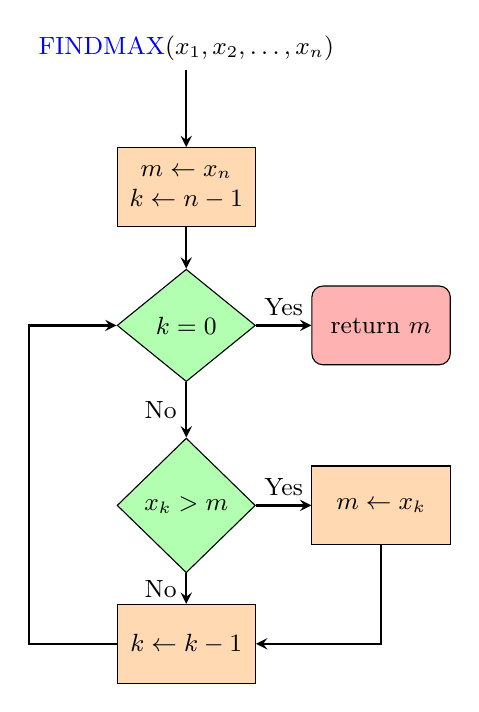
\begin{tikzpicture}[node distance=50pt]
          \small
          \node (head) {\textcolor{blue}{FINDMAX}$(x_1,x_2,\ldots,x_n)$};
          \node (init) [process, below of=head, align=center] {$m \leftarrow x_n$\\$k\leftarrow n-1$};
          \node (loop) [decision, below of=init] {$k = 0$};
          \node (return) [startstop, right = 20pt of loop] {return $m$};
          \node (newmax) [decision, below = 20pt of loop] {$x_k > m$};
          \node (update) [process, right = 20pt of newmax] {$m \leftarrow x_k$};
          \node (decrement) [process, below of = newmax] {$k \leftarrow k-1$};

          \draw [arrow] (head) -- (init);
          \draw [arrow] (init) -- (loop);
          \draw [arrow] (loop) -- node[anchor=east] {No} (newmax);
          \draw [arrow] (loop) -- node[anchor=south] {Yes} (return);
          \draw [arrow] (newmax) -- node[anchor=east] {No} (decrement);
          \draw [arrow] (newmax) -- node[anchor=south] {Yes} (update);
          \draw [arrow] (update) |- (decrement);
          \draw [arrow] (decrement) -- +(-2,0) |- (loop);
        \end{tikzpicture}
      }
      % 
      \colorbox[gray]{0.95}{
      \begin{minipage}{0.5\textwidth}
        \SetAlgoLined
        \begin{algorithm}[H]
          \DontPrintSemicolon
          \KwData{A sequence of numbers $(x_1, x_2,\ldots,x_n)$}
          \KwResult{ $\max\limits_{i=1}^{n}\ x_i$}
          
          $m \gets x_k$\;
          $k \gets n-1$\;
          \While {$k > 0$}
          {
            \If {$x_k > m$}
            {
              $m \gets x_k$\;
            }
            $k \gets k-1$\;
          }
          \Return $m$
          \caption{\small\color{blue} FINDMAX}
        \end{algorithm}
      \end{minipage}}
    \end{tabular}
  \end{center}

  The number of times that line 5 executes depends on the input sequence. Let us denote this quantity, i.e. the number of times that line 5 executes, as $L$. It is not difficult to see that $L$ ranges from $0$ (best case running time) to $(n-1)$ (worst case running time). But how realistic are these extreme cases? How probable is it to encounter these sequences?

  Given $n$ and assuming, \textit{wlog}, $\{x_1,x_2,\ldots,x_n\} = \{1,2,\ldots,n\}$, we can generate all possible sequences, and for each sequence, we can compute $L$. This allows us to tabulate how many sequences lead to each value of $L$. That is, we can compute, for each value of $i$ from $0$ to $n-1$, the number of sequences for which $L=i$. We can now find the average or expected value of $L$. We can also build a nice visualization, e.g. a bar chart.

\noindent\textbf{TASK}:  Using the above method, enter below the expected value of $L$ for different values of $n$ starting from $n=1$ and going up to as high a value of $n$ as you can manage. Show your working and explain any problems that you encounter. Also include a single visualization that meaningfully conveys as much information about the average cases as you can manage.

\noindent\textbf{TASK}:  Also share your visualization as a comment on the \textit{Week 01 Challenge} post in the course group on Yammer.

  \begin{solution}
    % Enter your solution here.
  \end{solution}


\end{questions}
\end{document}

%%% Local Variables:
%%% mode: latex
%%% TeX-master: t
%%% End:
